\documentclass[egilmezThesis.tex]{subfiles} 
\begin{document}
\chapter{Practical Application}
\label{chap:example}

In chapter \ref{chap:Justification} we introduce our own methodology for evaluating the similarity degree of fuzzy predicates. The method lacked a feature for realizing an error tolerance when working on knowledge bases with incomplete information. For that reason, three approaches are proposed in chapter \ref{chap:error}. The most elegant of these approaches, namely the \textit{Hybrid Approach} inherits the best features of the preceding ones, while avoiding the shortcomings via merging the two by attaining them some weights. Previously we displayed how these weights could be decided in an intuitionistic way, and hinted the possibility of an atomized procedure. In this chapter we show our proposal for atomizing the process with a real-world example.

\section{The Problem}
\label{problem}
In section \ref{chap:Introduction} we mention about how today's search engines have limited querying capabilities. We give the example of the query \textit{red car}, and say that an ideal frame work would return us the results of the query \textit{orange car} in addition to the original one, with lower credibility values. In the light of this, as our real-world practical example, we inspect the similarity relations between the colors. We may observe colors as a domain of interest in many distinct fields, however one particular interesting example is the set of canonical colors that the web browsers use, namely the \textit{X11 colors} \cite{Wri08}. The system makes use of the \textit{RGB} framework, where colors are specified as triplets. Every color is depicted by three values which represent the \textit{Red}, \textit{Green} and \textit{Blue} amount that the color consists of. The complete \textit{X11} table is shown in the following page.

\begin{center}
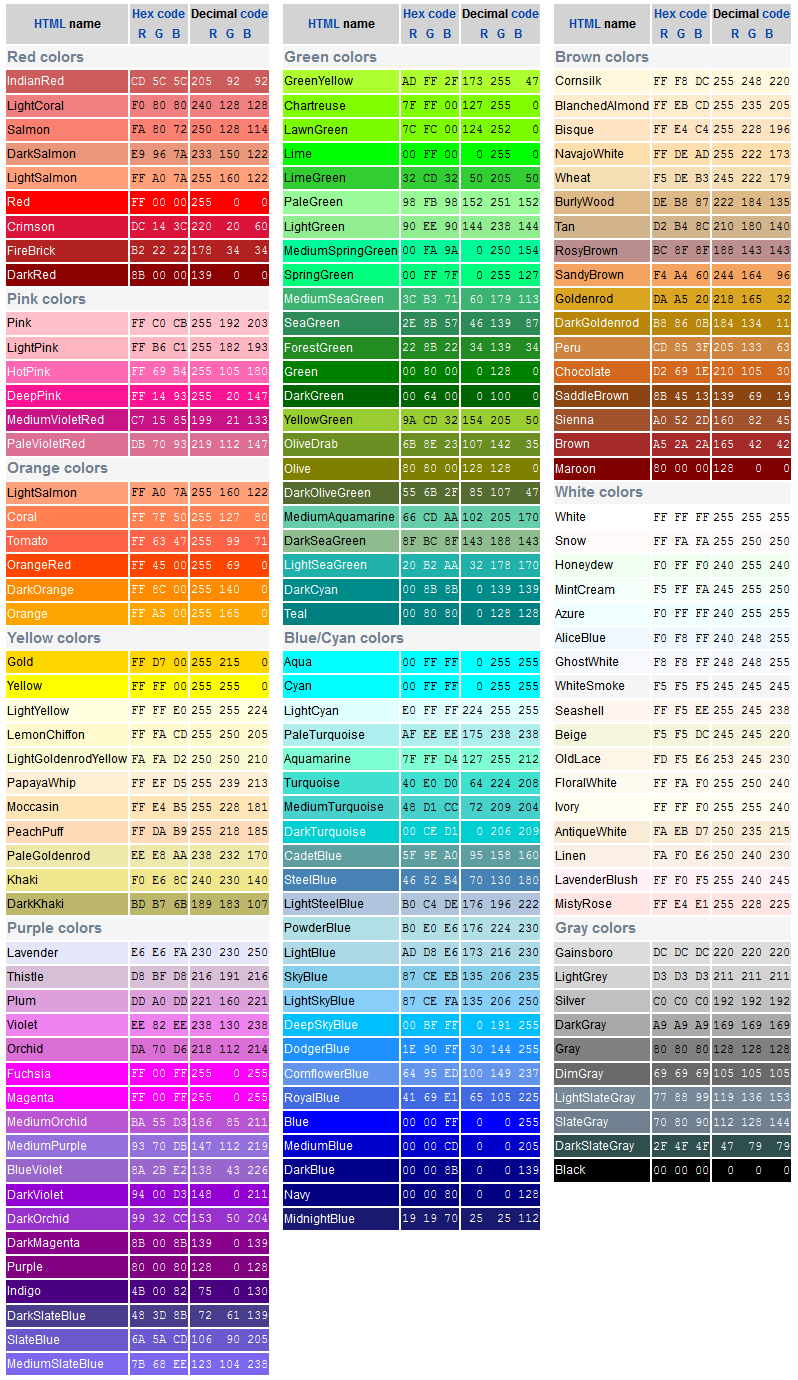
\includegraphics[width=1\textwidth]{misc/colorTable.png}
\end{center}

\subsection{Preliminaries}
\label{prem}
Before starting to proceed with the problem itself, we ought to mention about some problem specific concepts.

\subsubsection{Real World Similarity}
\label{rws}
As stated in section \ref{problem} in the \textit{RGB} scheme, all colors are represented by triplets of  \textit{Red}, \textit{Green} and \textit{Blue} values. With this in mind, when observing the similarity value between two colors, directly from the real-word data, we may consider them as if they were placed in \textit{3D space}. Thus each of the \textit{RGB} values acts as a coordinate for the corresponding color, and we may utilize a geometric distance formulation for this problem. In this scenario we adopt the \textit{Euclidean distance}, which is indeed one of the common definitions in the field of \textit{color science}. \cite{Sha02}

In Euclidean three-space, the distance between points $(x_1, y_1, z_1)$ and $(x_2, y_2, z_2)$ is
$$d=\sqrt{(x_2-x_1)^2+(y_2-y_1)^2+(z_2-z_1)^2}$$

Thus in our problem, the similarity distance between two colors $C$ and $S$ follows as:
$$similarity\_distance=\sqrt{(C_{Red}-S_{Red})^2+(C_{Green}-S_{Green})^2+(C_{Blue}-S_{Blue})^2}$$

We then follow by normalizing this metric distance value with the following algorithm

$$degree\_of\_similarity = 1 - \frac{similarity\_distance}{\sqrt{3*255^2}}$$
so that the resulting values fall between the \textit{real number} interval of $[0,1]$.

As one will notice the denominator of the function is the highest possible distance in the metric space. Real world correspondence of this scenario consists the color pair of \textit{Black} and \textit{White}. The algorithm would return $0$ as a result for this case. Moreover as expected, the pairing of any color with itself would result the algorithm computing $1$ as the similarity degree.

\subsubsection{Evaluated Similarity}
\label{evalSimPrac}

The gist of our methodology, which is introduced in chapter \ref{chap:MA}, is conserved in the practical case with minor modifications.

The predicate trees are relatively simple in structural terms. All are depth one, have three children.

\begin{figure}[h!]
\begin{center}
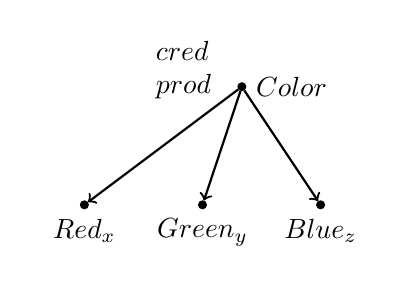
\begin{tikzpicture}[yscale=-1,
place/.style={circle,draw=black, fill=black, inner sep=0pt, 
              minimum size=1mm}]
\begin{scope}[xshift=4cm]
  \node[place] (1st) at (2, 0) [label=right: $Color$,
                                  label=left: 
     \begin{tabular}{l}
        $cred$\\
        $prod$\\
        $$\\  
     \end{tabular}
] {};

  \node[place] (2nd) at (0, 1.5) [label=below: $Red_x$,
                                  label=left:
     \begin{tabular}{l}
        $$\\
        $$\\
        $$\\  
     \end{tabular}
]{};
  \node[place] (3rd) at (1.5, 1.5)  [label=below: $Green_y$,
                                  label=left:
     \begin{tabular}{l}
        $$\\
        $$\\
        $$\\  
     \end{tabular}	] {}; 
  \node[place] (4th) at (3, 1.5)   [label=below: $Blue_z$,
                                  label=left:
     \begin{tabular}{l}
        $$\\
        $$\\
        $$\\  
     \end{tabular}
             ] {}; 
  
  %\node (dots) at (2,1.5) {$\cdots$};
	
  \draw[->, thick] (1st) -- (2nd);
  \draw[->, thick] (1st) -- (3rd);
  \draw[->, thick] (1st) -- (4th);
  
  \end{scope}

);
\end{tikzpicture}
\end{center}
\caption{Example of a color predicate tree}
\label{fig:ptEx}
\end{figure}
  
As we know main focus of our algorithm is utilizing predefined similarity relations between the subconcepts. In this particular example, we assume the only predefined similarity relations are the ones between the same \text{RGB} main colors. So for every $Red_\alpha$ and $Red_\beta$ a similarity relations is defined where $\alpha$ and $\beta$ are two integer values from the interval $[0, 255]$. 

The corresponding function is as follows:
$$similarity\_single\_color = 1 - \frac{|c_1-c_2|}{255}$$
  
which informally equals to the normalization of the metric distance on a single coordinate of the colors, so that it falls  into the interval of $[0,1]$.

Lastly, the evaluation function follows the same procedure described in chapter \ref{chap:MA}.



\subsubsection{Pseudo Credibility Values}
\label{pcv}

As discussed in chapter \ref{chap:error}, the main focus of interest is finding the weight constants in the \textit{Hybrid Approach(HA)} in an automatic sense. As one might observe, the problem consists the necessary information for calculating the values of \textit{VA} and \textit{EA} thus for fixing the weights, solely the credibility value should also be known. So for training weights, there is a need for some initial \textit{pseudo credibility values}.

In the end we want the product of our similarity and credibility estimation, close to the real degree of similarity.

$$  degree\_of\_similarity \times degree\_of\_credibility \cong real\_similarity $$

Through the preceding sections, we know evaluating both of values concerning similarities. So by putting these values in the equation, we may compute the variable of interest.


\subsubsection{Computing Weights}
\label{weights}

In section \ref{ha} we introduce the formula for the \textit{Hybrid Approach} as follows:

\begin{equation}
\textit{Credibility} = (w \times  \textbf{[Vertex\_Approach]}) + ((1-w) \times  \textbf{[Edge\_Approach]})
\end{equation}

where $w \in [0..1]$ .

As mentioned earlier, when one has the value of credibility, getting the value of the weights from the formula is trivial. 

One noteworthy concept here is the \textit{Global Weight}. The focus of this methodology is training the weights from some pre-given info, then fixing the weights through some procedure so the credibility values for new fuzzy rules can be determined. 

For maintaining the Multi-Adjoint properties as shown in \cite{MPS10}, we adopt the minimum operator for evaluating the global weight. Informally, we train a single weight for every similarity pair in our training set, then set the minimum of those values as our global weight.


\subsubsection{The Credibility}
\label{credPE}

When the weights are computed, the credibility values are easily evaluated via the function we introduce in section \ref{ha}. This consists the last step of the methodology, which could just be followed by checking both the credibility value and the similarity value together in comparison to the real degree of similarity.

Here the desired outcome is getting a conservative results, so to speak a value which does not exceed the original degree of similarity, but still finding one which is relatively close.

\section{A Practical Example}
\label{ape}

Suppose we have the following six color pairings in our training set:
\newline

\lstset{language=C++,basicstyle=\footnotesize}
\begin{lstlisting}[caption=The training set, breaklines=true]
Salmon Coral
Tomato Peru
YellowGreen MediumAquamarine	
FineBrick LightSeaGreen
Crimson RoyalBlue
Snow MidnightBlue
\end{lstlisting}

For the sake of an interesting display, let us select a pairing from the training set and one completely outside of the initial knowledge base, in order to construct our test set:
\newline

\lstset{language=C++,basicstyle=\footnotesize}
\begin{lstlisting}[caption=The training set, breaklines=true]
Tomato Peru
Pink Violet
\end{lstlisting}


With these  information in hand, we are ready for pursuing with the calculations.

\subsection{Training Process for Salmon and Coral}
\label{sc}

In this section we show step by step the process of training a weight via utilizing the info of a color pairing from the training set. The task is simply following the explicit process described in section \ref{prem}.

The first step is finding the real-world similarity proximity between the colors, namely \textit{Salmon} and \textit{Coral}. And for that, one needs to find out the metric distance of similarity of the colors.

We input the corresponding \textit{RGB} values of the colors into the modified euclidian function, defined in section \ref{rws}.

$$similarity\_distance=\sqrt{(C_{Red}-S_{Red})^2+(C_{Green}-S_{Green})^2+(C_{Blue}-S_{Blue})^2}$$

\begin{equation}
\begin{split}
similarity\_distance &= \sqrt{(C_{Red}-S_{Red})^2+(C_{Green}-S_{Green})^2+(C_{Blue}-S_{Blue})^2}\\
&= \sqrt{(C_{250}-S_{255})^2+(C_{128}-S_{127})^2+(C_{114}-S_{80})^2}\\
%&= \frac{1.05}{2}\\
&\cong{\textbf{34.38}}
\end{split} 
\end{equation}

Then use this metric distance value in the similarity evaluation function:

\begin{equation}
\begin{split}
degree\_of\_similarity &= 1 - \frac{similarity\_distance}{\sqrt{3*255^2}}\\
&= 1 - \frac{34.48}{\sqrt{3*255^2}}\\
%&= \frac{1.05}{2}\\
&\cong{\textbf{92.21}}
\end{split} 
\end{equation}


Second step of the process is finding the degree of similarity between the colors via using our own evaluation algorithm.  As we know first thing to do here is handling with the calculation of the similarity proximities of subconcepts. There will be three such relations that have to be taken into account. Let us compute one of them, namely the one concerning the \textit{Red} value of the colors:

\begin{equation}
\begin{split}
similarity\_single\_color &= 1 - \frac{|c_1-c_2|}{255}\\
&=1 - \frac{|250-255|}{255}\\
%&= \frac{1.05}{2}\\
&\cong{\textbf{0.98}}
\end{split} 
\end{equation}

After doing the same computation for the subconcept similarity relations regarding \textit{Green} and \textit{Blue}, and putting them in the evaluation function, we get:

$$degree\_of\_similarity = 0.947$$

In section \ref{pcv} we have stated that one we have the both results of the similarity evaluations, we may conclude the credibility value which will be used for training the weights. The corresponding formula and the computation is as follows:

\begin{equation}
\begin{split}
degree\_of\_similarity \times degree\_of\_credibility &= real\_similarity \\
degree\_of\_credibility &= \frac{real\_similarity}{degree\_of\_similarity} \\
&=1 - \frac{0.947}{0.98}\\
%&= \frac{1.05}{2}\\
&\cong{\textbf{0.973}}
\end{split} 
\end{equation}

The last computation enables us to continue with the last step of training, which is evaluating the weight.
In addition to the credibility value, the \textit{VA} and \textit{EA} values should also be calculated. Since all of the subconcepts are included in some similarity relation, the \textit{VA} value is $1$. Moreover as there are three predefined subconcept similarity relations out of nine possible relations(i.e. $3\times3 = 9$), the corresponding \textit{EA} value is $1/3$.

With the help of all these information, the so-called \textit{trained weight value} is:

\begin{equation}
\begin{split}
\textit{Credibility} &= (w \times  \textbf{[Vertex\_Approach]}) + ((1-w) \times  \textbf{[Edge\_Approach]})\\
w &= \frac{\textit{Credibility} -\textbf{[Edge\_Approach]}}{ \textbf{[Vertex\_Approach]} - \textbf{[Edge\_Approach]}}\\
%&= \frac{1.05}{2}\\
&=\frac{0.973-0.33}{1-0.33}\\
&\cong{\textbf{0.959}}
\end{split} 
\end{equation}

And this concludes our calculation for the first color pair of the training set.

\subsection{The Outcome}
\label{TCO}

A complete implementation of the process in \textit{C++} programming language is displayed at the appendix.

Regarding this example, the console output of the program is depicted in the following page.

As stated in section \ref{weights}, in order to preserve \textit{Multi-Adjoint} properties, we take the \textit{minumum} operation as the merging tool of the weight values from the training set.

By multiplying the credibility and the similarity  values evaluated from our algorithm, we compare the resulting number with the real similarity degree.

As can be seen in both examples, particularly both in the case of the example from the training set and also the newly introduced color pair, the results prove to be conservative. In other words they do not exceed the real values, which is a desired feature. In addition to that, we observe that the evaluated values are relatively close to the real-word correspondences. 

As both of these features are satisfied by the result of our methodology where a relatively small knowledge base is utilized, we consider our method to be displaying extreme promise for real world applications.

\newpage
\begin{center}
\label{The console output}
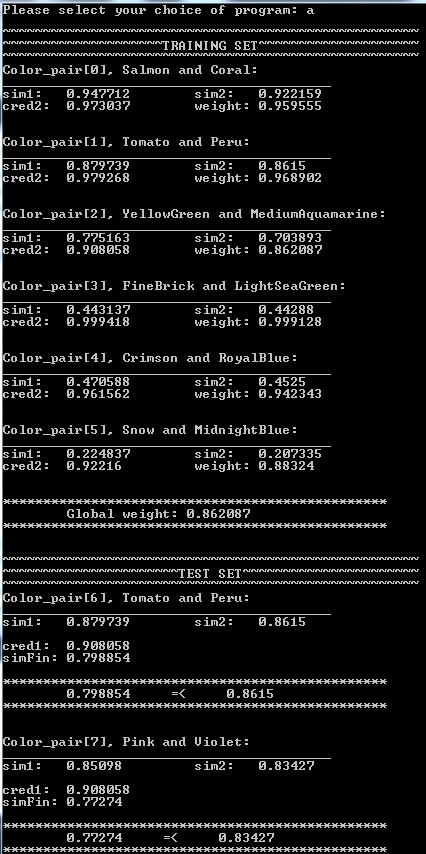
\includegraphics[width=0.73\textwidth]{console.jpg}
\end{center}

\end{document}